\newcommand{\code}[1]{\texttt{\textbf{#1}}}

\chapter{Introduction}\label{C:intro}

42 is a programming language created by Marco Servetto that is designed to be secure, easy to optimise and customisable \cite{servetto-2022A}.
\\[12pt]
Most modern, mainstream programming languages have features designed to prevent accidental errors from being introduced. For example, the static type system in Java is capable of producing compile-time errors in common cases of invalid code, which prevents those errors from causing bugs at runtime. 
\\[12pt]
The 42 language takes this idea further: it supports specifying arbitrary constraints, such as "names must start with an upper-case letter", or "these two lists must have the same length". When constraints like these are used in 42, the compiler can guarantee that those constraints will never be observed broken.
\\[12pt]
42 also supports fine-grained permissions, where parts of the program can specify what actions other parts will be able to perform. This can used be to, for example, prevent invalid data from being saved to a file or database. When one part of the program specifies constraints in this way, no other part of the code will be able to break them. With the compiler ensuring that the specified constraints are always enforced, large programs become safer, and easier to audit, while third-party libraries are less capable of potentially introducing security vulnerabilities.
\\[12pt]
Another unique feature of 42 is the ability to customise, extend or replace the standard library. While the default library, "Adam's Towel" \cite{servetto-2022B}, contains a wide selection of data types and methods, these can be further extended by users as needed.
\\[12pt]
The goal of this project is to demonstrate those constraints and security guarantees in practice. This is done by creating a public-facing website where users can submit arbitrary 42 code, that will then be executed in a constrained environment. Similar to a bug bounty programme, users will be encouraged to try and break the security guarantees of 42.




\chapter{Security Features in 42}\label{C:sec}

\section{Constraints}

A key feature of 42 is the ability to create constraints. Since constraints can contain arbitrary code, they can be used in a wide range of situations. Here is an example of a small 42 program that defines a “Point” class, with an invariant that both the x- and y-coordinates must always be positive:

\begin{mylisting}{Simple Constraint}
reuse [L42.is/AdamsTowel]

Point = Data:{
  Double x
  Double y

  @Cache.Now
  class method Double distanceFromOrigin(Double x, Double y) = 
    ((x*x)+(y*y)).pow(exp=\"0.5")

  // x and y must always be positive
  @Cache.Now
  class method Void invariant(Double x, Double y) = 
    if !(x>=0Double && y>=0Double) error X"""%
      | Invalid state:
      | x = %x
      | y = %y
      """
  }

Main=(
  Point p = Point(x=Double"5", y=Double"3")
  // This would result in an error:
  //Point p2 = Point(x=Double"5", y=Double"-3")
  Debug(S"p = %p")
  )
\end{mylisting}

In this program, in addition to defining a \code{Point} class in much the same way as one would in Java, we have created an additional "\code{invariant}" method, annotated with "\code{@Cache.Now}. The annotation causes 42 to automatically call this method whenever an instance of \code{Point} is created. The method itself throws an error if \code{x} or \code{y} have unexpected values, and the compiler ensures that this constraint is checked both when a Point instance is constructed, and also whenever instances are modified.
\\[12pt]
If an exception does get thrown due to the invariant being broken, it can still be caught, but 42 ensures that no part of the code will ever be able to access a \code{Point} instance with a broken constraint.
\\[12pt]
While the previous example used a \code{Point} class with immutable fields, constraints can also be used with fully mutable fields, like in this example:

\begin{mylisting}{Constraint with mutable fields}
reuse [L42.is/AdamsTowel]
Point = Data:{
  // `var` makes the `x` and `y` values modifiable
  var Double x
  var Double y
  mut method Void add(Double dx) = 
    this.x(this.x() + dx)
  @Cache.Now class method Void invariant(Double x, Double y) = 
    if x < 0Double || y < 0Double error X"""%
      | Invalid state:
      | x = %x
      | y = %y
      """
  }

Main=(
  mut Point p = Point(x=Double"5", y=Double"3")
  // now we can try to mutate `x`:
  p.add(dx=Double"-6") // error on this line
  Debug(S"p = %p")
  )
\end{mylisting}

This third example shows how to catch a constraint error:

\begin{mylisting}{Catching a constraint error}
reuse [L42.is/AdamsTowel]
Point = Data:{
  // `var` makes the `x` and `y` values modifiable
  var Double x
  var Double y
  mut method Void add(Double dx) = 
    this.x(this.x() + dx)
  @Cache.Now class method Void invariant(Double x, Double y) = 
    if x < 0Double || y < 0Double error X"""%
      | Invalid state:
      | x = %x
      | y = %y
      """
  }

Main=(
  mut Point p = Point(x=Double"5", y=Double"3")
  // now we can try to mutate `x`:
  p.add(dx=Double"-6") // error on this line
  catch error This.X msg1 (
     Debug(S"We got an error: %msg1")
     )
  Debug(S"p = %p")
  )
\end{mylisting}

It prints the following output:
\begin{mylisting}{Constraint error}
We got an error:
Message This.X(This.Message, This.HasToS, This.Message.Assert):
 Invalid state:
 x = -1.0
 y = 3.0

\end{mylisting}

\section{Mutability}

TODO: Explain 'mut', 'imm', etc. keywords and how they are enforced

\chapter{Bug Bounty Programmes}

Software has become significantly more complex. It?s become ever easier to add third-party libraries and dependencies to software projects, any of which can add security vulnerabilities to existing code. The size of software projects, measured in lines of code, has continued to grow. For example, the initial 1.0 release of Linux comprised of approx. 180,000 lines of code \cite{mccandless-2020, perry-2012}, whereas in 2020 the kernel had grown to more than 27 million \cite{larabel-2020}. The increased use of third-party libraries comes hand-in-hand with an increase in contributor numbers, which raises the risk of supply-chain attacks \cite{sharma-2021}. Another example of a recent high-profile security vulnerability is the Log4J vulnerability \cite{apache-2021}, which led to arbitrary code execution and had hundreds of thousands of exploit attempts within days of being publicised \cite{raveendran-2021}.
\\[12pt]
Bug Bounty programmes are one technique to incentivise the general public to help search for security bugs. They enable individuals to receive compensation and recognition for finding such bugs. The first bug bounty programme started in 1983 \cite{hackerone-2017}, where anyone finding a bug in the VRTX operating system would receive a VW Beetle as compensation \cite{hunter-ready-inc-1983}. They are often used in combination with existing best practices like code reviews, pen tests, automated scanning, and security audits by third-party cybersecurity companies.
\\[12pt]
A current example of a bug bounty programme is Microsoft, which pays up to US\$250,000 in the case of Hyper-V remote code execution \cite{microsoft-2022}. Google has a similar program, with a maximum amount of US\$1,000,000 for Android vulnerabilites \cite{google-2022} and Apple similarly pays up to US\$1 million for kernel code execution bugs \cite{apple-inc-2022}.
\\[12pt]
In 2018 Facebook paid out \$50,000 to one person for finding a bug that exposed private user data \cite{newman-2018}. The vulnerability made it possible to see who liked or commented on particular posts on Facebook. Facebook has more than 2 billion active users \cite{datareportal-2022}, any of whom could have had their private data exposed as part of an attack using this vulnerability. Not only oppressive regimes, but also employers and other third-parties might have been able to access this sensitive data.
\\[12pt]
42 is a language designed for high security. It supports constraints and invariants to enforce restrictions on parts of the code. For example, the 42 compiler makes it possible to include third-party code, but only give it limited permissions. File system or memory access can be restricted on a granular basis, which makes it considerably safer compared to other programming languages. However, these restrictions need to be implemented correctly in the compiler, which is a comparatively small project on a limited budget. A bug bounty programme for the 42 compiler could therefore be useful in increasing security similar to the programmes listed above.

\begin{figure}[h]
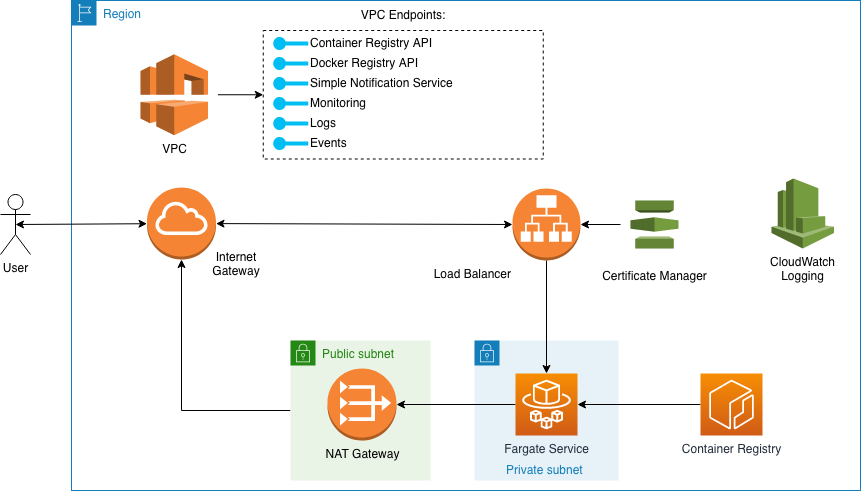
\includegraphics[width=\textwidth]{../diagrams/ecs-fargate.drawio.png}
\caption{Architecture for our ECS Fargate solution}
\end{figure}